%
% File acl2014.tex
%
% Contact: giovanni.colavizza@epfl.ch
%%
%% Based on the style files for ACL-2013, which were, in turn,
%% Based on the style files for ACL-2012, which were, in turn,
%% based on the style files for ACL-2011, which were, in turn,
%% based on the style files for ACL-2010, which were, in turn,
%% based on the style files for ACL-IJCNLP-2009, which were, in turn,
%% based on the style files for EACL-2009 and IJCNLP-2008...

%% Based on the style files for EACL 2006 by
%%e.agirre@ehu.es or Sergi.Balari@uab.es
%% and that of ACL 08 by Joakim Nivre and Noah Smith

\documentclass[11pt]{article}
\usepackage{acl2014}
\usepackage{times}
\usepackage{url}
\usepackage{latexsym}

\usepackage{subcaption}

\usepackage[margin=1in]{geometry}
\usepackage{amsmath,amsthm,amssymb, graphicx, multicol, array}

%\setlength\titlebox{5cm}

% You can expand the titlebox if you need extra space
% to show all the authors. Please do not make the titlebox
% smaller than 5cm (the original size); we will check this
% in the camera-ready version and ask you to change it back.


\title{Official work with private tools}

\author{Rehan Mulakhel \\
  {\tt \{rehan.mulakhel\}} \\\And
  Brice Repond \\
  {\tt \{brice.repond\}} \\\And
  Kenneth Nguyen \\
{\tt \{kenneth.nguyen\}\{@epfl.ch\}} \\}

\date{}

\begin{document}
\maketitle
\begin{abstract}
Identifying topics from a relatively large amount of textual messages could not be done efficiently a few decades ago. In this paper, we will compare results obtained from a naive algorithm based on key words system coupled with external knowledge against traditional machine learning to better understand the sensitive and sometimes confidential information contained in Hillary Clinton's emails.
\end{abstract}

\section{Introduction}

The Hillary Clinton email controversy arising from the use of private email server for official communications during her tenure as Secretary of State hit the headline of the media in 2015. However the content of the emails was not covered properly and reading relevant information related to it remains a difficult task. We will use the content of the emails and the network of the connection to draw conclusions.

\section{Datasets description}

Kaggle provides the same data in two different formats: four csv files VS one sqlite file. We only consider the former because the operations we will perform require the built in functions of pandas. The raw data with dimensions have the following shapes:

\begin{itemize}
    \item \texttt{emails.csv} (7945, 22)
    \item \texttt{persons.csv} (513, 2)
    \item \texttt{aliases.csv} (850, 3)
    \item \texttt{email\_receiver.csv} (9306, 3)
\end{itemize}

Theses tables form an entity relationship diagram. One would expect the emails to be linked somehow to the persons and the persons to be linked to the aliases. However, the raw data is based on the fields of the emails rather than the structure of a well designed database. Indeed, emails fields use (textual!) aliases to join the tables. Therefore, it is not possible to get the value of the persons directly from the emails.

The reasons for this inconvenient choice is likely due to the fact that the data were generated before the creation of the structure storing it. The one who gathered the data stopped the process at an early stage, leaving us to fend ourselves. Actually, the few extracted values such as the content are not useful because of the poor quality.

\section{Data exploration}

In general, it is not possible to organize the work in a cascade fashion when working with potentially dirty data. Going back and forth cannot be avoided and is required to understand the data. Understanding the data is necessary to improve the cleaning actions or to recover from missing or unusable values. There are easy mistakes or bad design choice we can observe by simply over reading columns. There are hidden mistakes which cannot be spot without carefully reading and \emph{expecting} some values. We describe the recovering process of the missing and/or dirty fields in the notebook.

\subsection{Emails}

The subject of an email cannot always be deduced from its content because all messages have an implicit context. The same sentence does not necessarily have the same meaning all the time. It depends on too many parameters like the person who wrote it and the moment when it was written and the social conventions at the time when it was written...

\subsubsection{Distribution over time}

\begin{figure}[h]
	\centering
	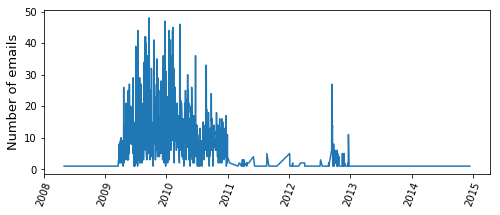
\includegraphics[width=\linewidth]{images/emails_distribution.png}
	\caption{Time distribution of all the emails}
	\label{fig:emails_time_distribution}
\end{figure}

The Figure \ref{fig:emails_time_distribution} shows three periods we call `contexts' we identify them as:

\begin{itemize}
    \item \texttt{ctx0} from 2009 to 2011
    \item \texttt{ctx1} from 2011 to 2012 June
    \item \texttt{ctx2} from 2012 June to 2013
\end{itemize}

We should keep in mind that some emails may have not been or could have not been disclosed.

It is hard to give an interpretation without introducing external knowledge. We can map the second periods to the Libya intervention in 2011 and the third one to the murder of US ambassador in Libya.

\subsubsection{Sender and Receiver}
\label{sec:sender_receiver}

The number of persons in the network is roughly $300$ after recovering dirty values. The frequency of the messages sent or received changes in time. The topics and words changes too as we will see in section~\ref{sec:topics_detection}. However, we see in Figure~\ref{fig:network_evolution} some names appear in the three contexts. Actually, these nodes are mostly political advisers of Hillary Clinton and they are the strongest links in the network.

\begin{figure*}[!t]
	\centering
	\begin{subfigure}[b]{0.3\linewidth}
		\centering
		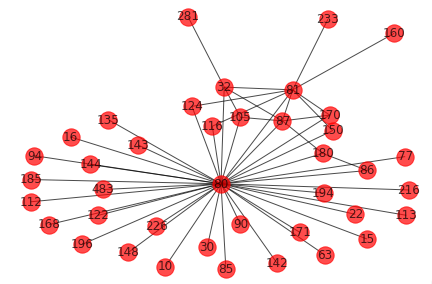
\includegraphics[width=\linewidth]{images/network_ctx0.png}
		\caption[]%
		{{\small \texttt{ctx0} with $w(e) \geq 8$}}    
		\label{fig:network_ctx0}
	\end{subfigure}
	\begin{subfigure}[b]{0.3\linewidth}
		\centering
		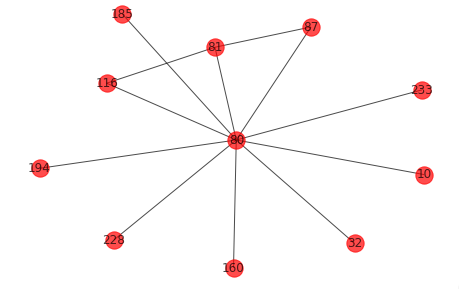
\includegraphics[width=\linewidth]{images/network_ctx1.png}
		\caption[]%
		{{\small \texttt{ctx1} with $w(e) \geq 0$}}  
		\label{fig:network_ctx1}
	\end{subfigure}
	\begin{subfigure}[b]{0.3\linewidth}
		\centering
		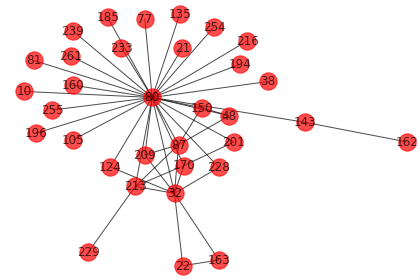
\includegraphics[width=\linewidth]{images/network_ctx2.png}
		\caption[]%
		{{\small \texttt{ctx2} with $w(e) \geq 0$}}
		\label{fig:network_ctx2}
	\end{subfigure}
	\caption{The evolution of Hillary's network from 2009 to 2013.}
	\label{fig:network_evolution}
\end{figure*}

\subsubsection{Content}

A typical email is composed of a sender, a receiver, a time stamp and a content. Some emails are made of many replies. Sometimes the replies come from the same person. We decided to keep those emails as single emails. This will not hurt the results too much since the thread of conversations should be related to the same topics in most cases.

During the pre-process, we remove the unnecessary lines and common words which appear in all emails. We keep only sentences having at least three words and join them with the char `$|$'.

During the post-process, we remove the frequent words by setting the threshold of the tf-idf at 3.4. We got this value by manually testing and observing the output of the words which would be removed.

\section{Topics detection}
\label{sec:topics_detection}

The size of the dataset is too small to get valid results using common machine learning tools. We have $|\{ emails \}| << |\{ words \}|$. On the other hand, there are potentially a huge number of topics appearing in the few emails we have. The conditions are met for an overfit. We will use two different techniques to discover information: one basic and naive way based on key words, and one more complex based on logistic regression, hoping to reach the same conclusions.

\subsection{Key words}

Enriching data is a common task in data science. It could be useful to map an email to one or many places on the Earth. We consider the following: North America, Latino world, Europe, Africa, Middle East, Central Asia, Far East, Russia (including Ukraine). Each of these columns is a boolean and one email can be situated in more than a single place. One naive system can determine the position based on some key words appearing in the content of the emails. The results of this solution need to be taken with cautious because it contains a lot of false positive when frequent words are used as key words, and a lot of false negative when important words are missing. For our case, we can expect `Obama' to appear frequently even when the content is not related to the United States.

\subsubsection{Emails distribution per region}

If we consider all the dataset and not the feature `North America', emails are dominated by the Middle East and Europe, followed by Central Asia, Far East then Africa. Latino world and Russia do not seem to be concern to much by the emails compared to the others. We will neglect that and consider only the distribution within what we call \texttt{ctx} as shown in Figure~\ref{fig:map_distribution_evolution}.

\begin{figure*}[!t]
	\centering
	\begin{subfigure}[b]{0.3\linewidth}
		\centering
		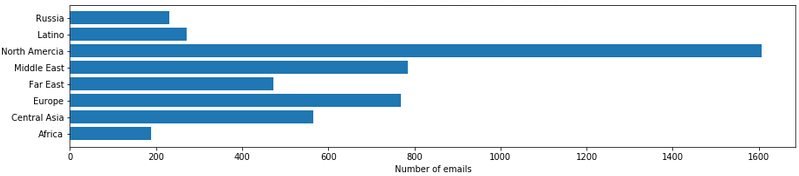
\includegraphics[width=\linewidth]{images/emails_map_ctx0.png}
		\caption[]%
		{{\small Distribution in \texttt{ctx0}}}    
		\label{fig:emails_map_distribution_ctx0}
	\end{subfigure}
	\begin{subfigure}[b]{0.3\linewidth}
		\centering
		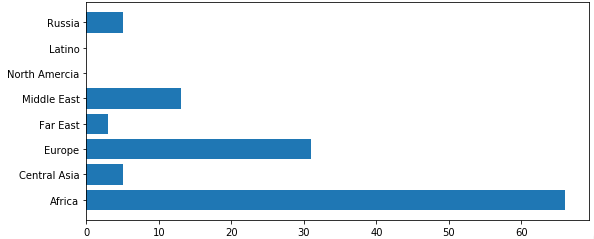
\includegraphics[width=\linewidth]{images/emails_map_ctx1.png}
		\caption[]%
		{{\small Distribution in \texttt{ctx1}}}
		\label{fig:emails_map_distribution_ctx1}
	\end{subfigure}
	\begin{subfigure}[b]{0.3\linewidth}
		\centering
		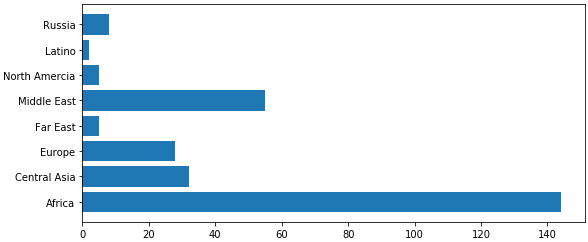
\includegraphics[width=\linewidth]{images/emails_map_ctx2.png}
		\caption[]%
		{{\small Distribution in \texttt{ctx2}}}
		\label{fig:emails_map_distribution_ctx2}
	\end{subfigure}
	\caption{The evolution of emails distribution from 2009 to 2013 based on key words.}
	\label{fig:map_distribution_evolution}
\end{figure*}

If we take the plot in Figure \ref{fig:emails_map_distribution_ctx0}, then it not surprising to observe the same distribution as the one we have for the whole dataset. It is because the majority of emails were sent during this moment. What is surprising is the share Europe takes.

For the \texttt{ctx1} in Figure \ref{fig:emails_map_distribution_ctx1}, the dominating place is Africa, followed by Europe then Middle East.

For the last context in Figure \ref{fig:emails_map_distribution_ctx2}, we see that Africa is again dominating but Middle East beats Europe.

The plots based on key words lead us to the hypothesis we have drawn based on the distribution of the emails date. Indeed, Europe looses width from \texttt{ctx1} to \texttt{ctx2} against Africa. It seems safe to consider NATO operation in Libya as the main topic in the middle.

\subsubsection{Word cloud and $N$-grams}

We create clouds to observe the dominant terms in each context in Figure~\ref{fig:word_cloud}. Unfortunately, it does not help much for the \texttt{ctx0}. However, it confirms our hypothesis: \texttt{ctx1} is related to Libya and `quaddafi' while \texttt{ctx2} is related Libya and `embassi' (because of the stemming process).

\begin{figure*}[!t]
	\centering
	\begin{subfigure}[b]{0.45\linewidth}
		\centering
		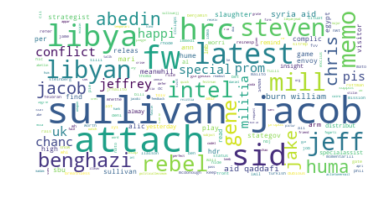
\includegraphics[width=\linewidth]{images/word_cloud_ctx1.png}
		\caption[]%
		{{\small Word cloud for \texttt{ctx1}}}
		\label{fig:word_cloud_ctx1}
	\end{subfigure}
	\begin{subfigure}[b]{0.45\linewidth}
		\centering
		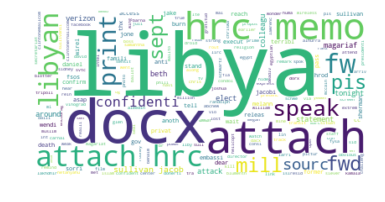
\includegraphics[width=\linewidth]{images/word_cloud_ctx2.png}
		\caption[]%
		{{\small Word cloud for \texttt{ctx2}}}
		\label{fig:word_cloud_ctx2}
	\end{subfigure}
	\caption{Words dominating in each context.}
	\label{fig:word_cloud}
\end{figure*}

We can do better using the $n$-grams. We arbitrary decided to choose $n = 2$. This time we apply the algorithm on the regions rather than the contexts.

\begin{description}
	\item[Africa] Human rights, Libya, policy transition, revolution of 2011.
	\item[Central Asia] Human rights, Al Qaida, Ben Laden. Pakistan, Saudi Arabia.
	\item[Europe] Climate change, European Union, UK, human rights.
	\item[Far East] Petrol, climate change, human rights. Related to specific countries as North Korea, South Korea, Saudi Arabia.
	\item[Middle east] Human rights, peace, missile defense. Related to Israel, Palestine.
	\item[North America] Health care, human rights are some subjects.
	\item[Latino] Contains only around 250 emails about subjects completely different.
	\item[Russia] Missile defense, human rights, North Korea, arm control are some interesting subjects.
\end{description}

Human rights occur frequently in the documents. It is likely linked to the fact that the majority of emails are produced by her political advisers as we have seen in Section~\ref{sec:sender_receiver}, who express themselves in diplomatic terms.

One final word on the words... We have not seen anything related to Wikileaks yet. It is hard to think Julian Assange name or work were not discussed. Actually, Wikileaks appears in the word cloud per region for Europe, Russia, Middle East, Central Asia and Far East.

\subsection{Machine learning}

Document clustering and topics extraction can be done using unsupervised machine learning algorithm. We visualize the clusters in Figure~\ref{fig:dendograms} where we group \emph{emails}. The \texttt{ctx0} is not computed because it contains to many elements.

\begin{figure*}[!t]
	\centering
	\begin{subfigure}[b]{0.4\linewidth}
		\centering
		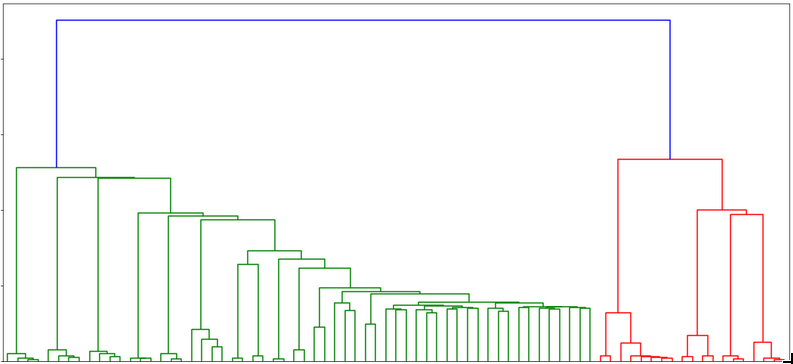
\includegraphics[width=\linewidth]{images/dendogram_ctx1.png}
		\caption[]%
		{{\small Emails clusters in \texttt{ctx1}}}
		\label{fig:dendogram_ctx1}
	\end{subfigure}
	\begin{subfigure}[b]{0.4\linewidth}
		\centering
		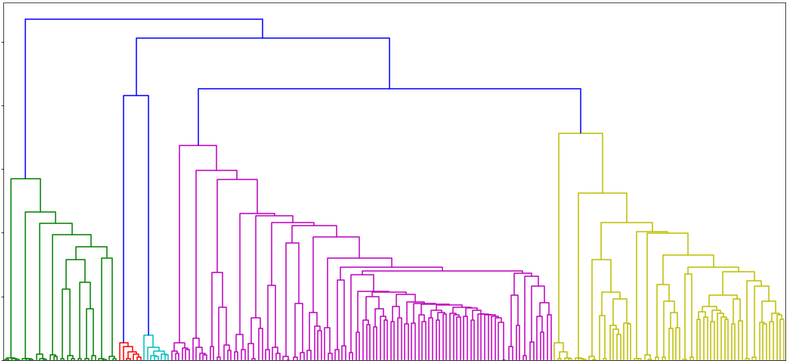
\includegraphics[width=\linewidth]{images/dendogram_ctx2.png}
		\caption[]%
		{{\small Emails clusters in \texttt{ctx2}}}
		\label{fig:dendogram_ctx2}
	\end{subfigure}
	\caption{Dendograms grouped documents by cosine distance.}
	\label{fig:dendograms}
\end{figure*}

We know how to extract topics from different books. We will simply adapt our case to make it work. We create our `books' by concatenating \emph{sentences} within the same context.

The inputs of our linear regression are not emails but sentences. The target value will be the three contexts we observe in Figure~\ref{fig:emails_time_distribution}. The goal is to learn the topics covered in each context. The regularization parameter is taken at the moment when we see the (cross validation) score decreasing. The result we get are the following:

\begin{description}
    \item[Context 0] Afghanistan, China, Iraq
    \item[Context 1] Libya (Qaddafi, NATO, fight, rebel), Egypt (Morsi)
    \item[Context 2] US Ambassador killed in Benghazi, Morocco, Tunisia, Islam and Muslim (due to the movie Innocence of Muslims), Romney
\end{description}

These topics are convincing. The Figure~\ref{fig:dendogram_ctx1} shows two classes. One of them is likely to be related to North Africa which includes Libya (NATO, fly zone, ...). We can suppose the other class is related to Mohamed Morsi. We can also suppose Egypt and Libya are in the same cluster and the other one contains topics unrelated to this part of the world and unrelated to each other too.

The Figure \ref{fig:dendogram_ctx2} shows at least two topics dominating. We guess there is one cluster containing emails related to the murder of the US ambassador. Another one probably contains events related directly or indirectly to the movie `Innocence of Muslims'.

\section{Conclusion}

The naive algorithm based on key words works surprisingly well in this specific case. But it requires a lot of external knowledge and is prone to miss interesting information. On the other hand, the unsupervised algorithm is easier to implement and produces results which are more easy to interpret. In both cases, external knowledge helps to understand the context.

It is feasible to split the emails into private and professional category by identifying the personal contacts in the network. Running the unsupervised algorithms could display embarrassing information. In the end, it is a bad idea to mix private and professional tools which can lead to dangerous leaks. This may also reduce the number of burn out and improve the well-being of people. But this is another subject.

\end{document}
